\documentclass[tikz,border=10pt]{standalone}
\usepackage{tikz}
\usepackage{amssymb}
\usetikzlibrary{shapes.geometric, arrows.meta, positioning, fit, backgrounds, calc, shadows.blur, decorations.pathreplacing}

% --- Color Definitions (Google Material Palette) ---
\definecolor{greenFill}{HTML}{E8F5E9}
\definecolor{greenStroke}{HTML}{43A047}
\definecolor{memFill}{HTML}{FFF3E0}
\definecolor{memStroke}{HTML}{FFB74D}
\definecolor{coreFill}{HTML}{E1F5FE}
\definecolor{coreStroke}{HTML}{0277BD}
\definecolor{optFill}{HTML}{FCE4EC}
\definecolor{optStroke}{HTML}{E91E63}
\definecolor{procFill}{HTML}{FFF9C4}
\definecolor{procStroke}{HTML}{FBC02D}
\definecolor{purpleFill}{HTML}{F3E5F5}
\definecolor{purpleStroke}{HTML}{7B1FA2}

\begin{document}

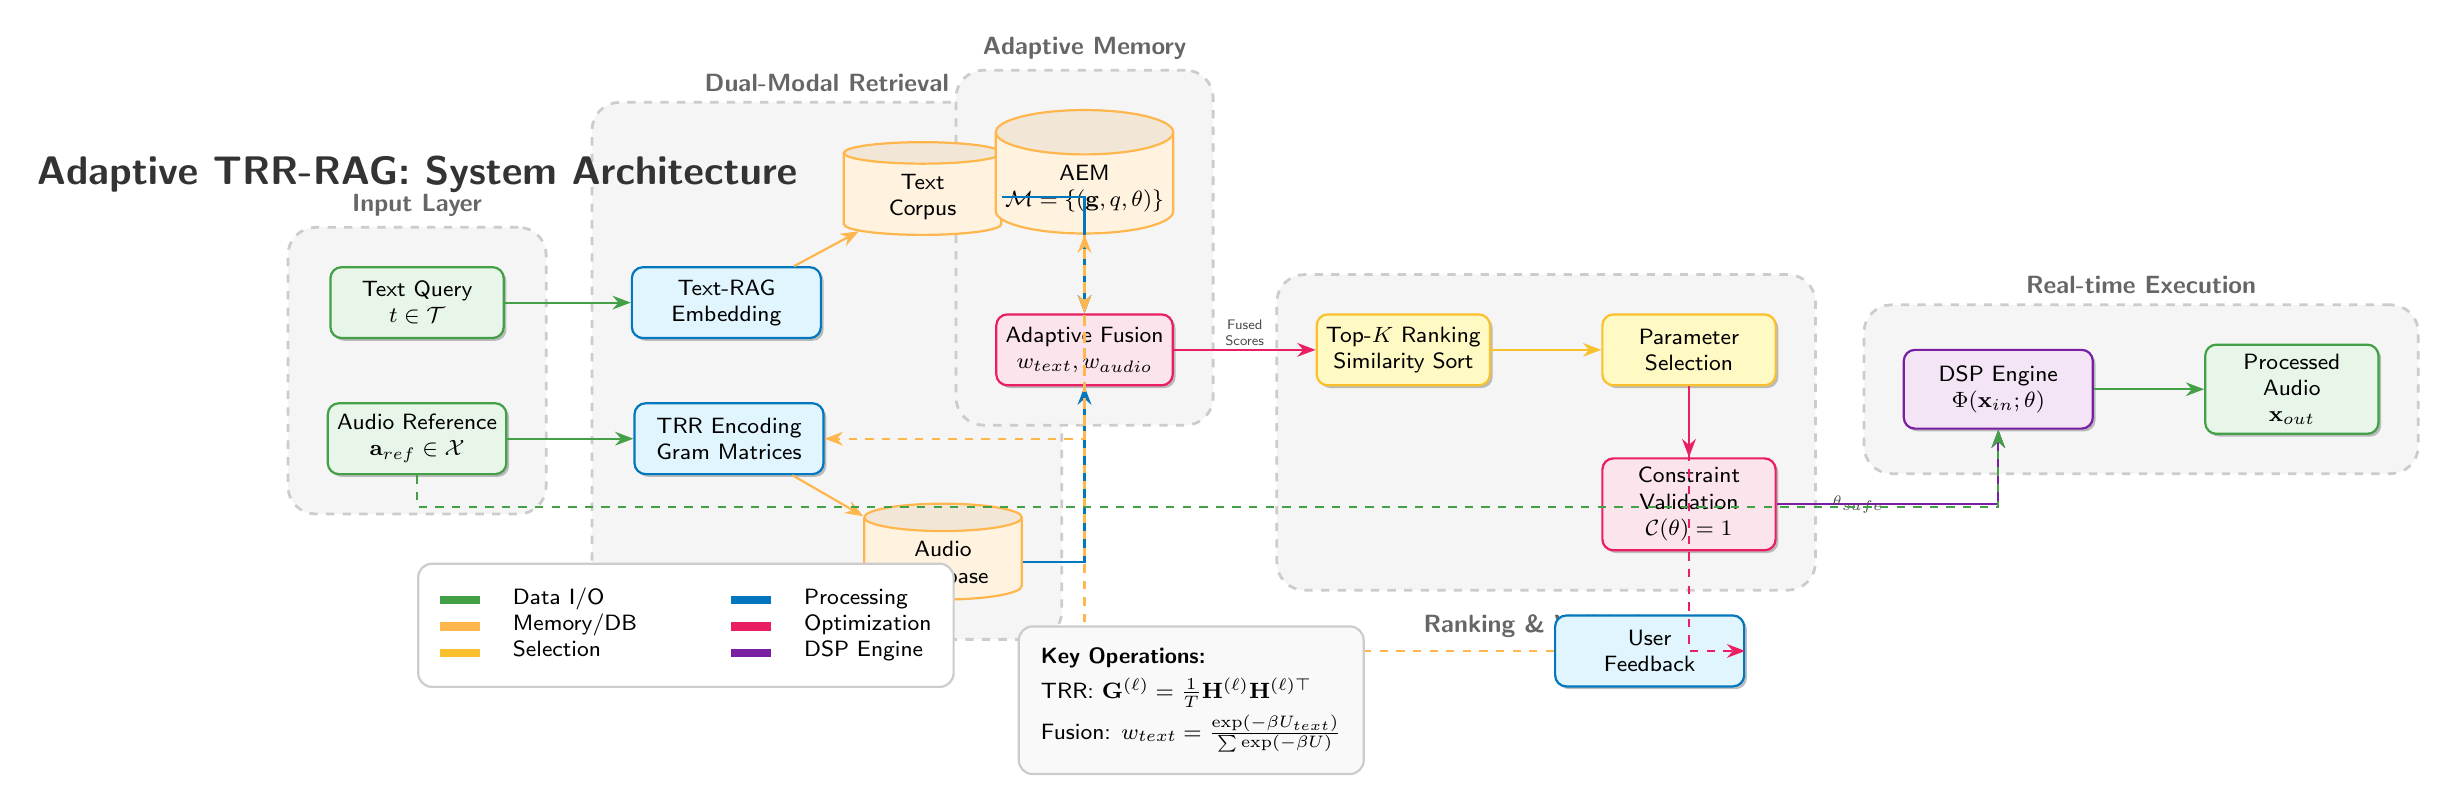
\begin{tikzpicture}[
    node distance=1.0cm and 1.4cm,
    font=\sffamily\footnotesize,
    >=Stealth,
    thick,
    % --- Styles ---
    dataNode/.style={
        rectangle, rounded corners=4pt,
        draw=greenStroke, thick,
        fill=greenFill,
        minimum width=2.2cm, minimum height=0.9cm,
        align=center,
        drop shadow={shadow blur steps=5, shadow xshift=1pt, shadow yshift=-1pt}
    },
    memNode/.style={
        cylinder, cylinder uses custom fill,
        cylinder body fill=memFill, cylinder end fill=memFill!90!gray,
        shape border rotate=90,
        aspect=0.25,
        draw=memStroke, thick,
        minimum width=2.0cm, minimum height=1.1cm,
        align=center
    },
    opNode/.style={
        rectangle, rounded corners=4pt,
        draw=coreStroke, thick,
        fill=coreFill,
        minimum width=2.4cm, minimum height=0.9cm,
        align=center,
        drop shadow={shadow blur steps=5, shadow xshift=1pt, shadow yshift=-1pt}
    },
    optNode/.style={
        rectangle, rounded corners=4pt,
        draw=optStroke, thick,
        fill=optFill,
        minimum width=2.2cm, minimum height=0.9cm,
        align=center,
        drop shadow={shadow blur steps=5, shadow xshift=1pt, shadow yshift=-1pt}
    },
    procNode/.style={
        rectangle, rounded corners=4pt,
        draw=procStroke, thick,
        fill=procFill,
        minimum width=2.2cm, minimum height=0.9cm,
        align=center,
        drop shadow={shadow blur steps=5, shadow xshift=1pt, shadow yshift=-1pt}
    },
    dspNode/.style={
        rectangle, rounded corners=4pt,
        draw=purpleStroke, thick,
        fill=purpleFill,
        minimum width=2.4cm, minimum height=1.0cm,
        align=center,
        drop shadow={shadow blur steps=5, shadow xshift=1pt, shadow yshift=-1pt}
    },
    group/.style={
        draw=gray!40, dashed, rounded corners=10pt,
        inner sep=14pt, fill=gray!8,
        line width=1pt
    },
    edgeLabel/.style={
        font=\sffamily\tiny,
        text=black!70,
        align=center,
        inner sep=1pt
    }
]

% --- INPUT LAYER ---
\node[dataNode] (textInput) {Text Query\\$t \in \mathcal{T}$};
\node[dataNode, below=0.8cm of textInput] (audioInput) {Audio Reference\\$\mathbf{a}_{\text{ref}} \in \mathcal{X}$};

% --- RETRIEVAL MODULE ---
\node[opNode, right=1.6cm of textInput] (textRAG) {Text-RAG\\Embedding};
\node[opNode, right=1.6cm of audioInput] (trr) {TRR Encoding\\Gram Matrices};

% --- KNOWLEDGE BASES ---
\node[memNode, above right=0.4cm and 0.8cm of textRAG] (textKB) {Text\\Corpus};
\node[memNode, below right=0.4cm and 0.8cm of trr] (audioKB) {Audio\\Database};

% --- FUSION ---
\node[optNode, right=2.2cm of textRAG, yshift=-0.6cm] (fusion) {Adaptive Fusion\\$w_{\text{text}}, w_{\text{audio}}$};

% --- MEMORY ---
\node[memNode, above=1.0cm of fusion] (memory) {AEM\\$\mathcal{M} = \{(\mathbf{g}, q, \theta)\}$};

% --- RANKING & SELECTION ---
\node[procNode, right=1.8cm of fusion] (ranking) {Top-$K$ Ranking\\Similarity Sort};
\node[procNode, right=1.4cm of ranking] (selection) {Parameter\\Selection};

% --- CONSTRAINT CHECK ---
\node[optNode, below=0.9cm of selection] (constraint) {Constraint\\Validation\\$\mathcal{C}(\theta) = 1$};

% --- DSP ENGINE ---
\node[dspNode, right=1.6cm of selection, yshift=-0.5cm] (dsp) {DSP Engine\\$\Phi(\mathbf{x}_{\text{in}}; \theta)$};

% --- OUTPUT ---
\node[dataNode, right=1.4cm of dsp] (output) {Processed\\Audio\\$\mathbf{x}_{\text{out}}$};

% --- FEEDBACK LOOP ---
\node[opNode, below=0.8cm of constraint, xshift=-0.5cm] (feedback) {User\\Feedback};

% --- ARROWS: Input to Processing ---
\draw[->, color=greenStroke] (textInput) -- (textRAG);
\draw[->, color=greenStroke] (audioInput) -- (trr);

% --- ARROWS: Processing to KB ---
\draw[->, color=memStroke] (textRAG) -- (textKB);
\draw[->, color=memStroke] (trr) -- (audioKB);

% --- ARROWS: KB to Fusion ---
\draw[->, color=coreStroke] (textKB) -| (fusion);
\draw[->, color=coreStroke] (audioKB) -| (fusion);

% --- ARROWS: Memory ---
\draw[->, color=memStroke, dashed] (memory) -- (fusion);
\draw[->, color=memStroke, dashed] (memory) |- (trr);

% --- ARROWS: Fusion to Ranking ---
\draw[->, color=optStroke] (fusion) -- (ranking) node[midway, edgeLabel, above] {Fused\\Scores};

% --- ARROWS: Ranking to Selection ---
\draw[->, color=procStroke] (ranking) -- (selection);

% --- ARROWS: Selection to Constraint ---
\draw[->, color=optStroke] (selection) -- (constraint);

% --- ARROWS: Constraint to DSP ---
\draw[->, color=purpleStroke] (constraint) -| (dsp) node[pos=0.25, edgeLabel, left] {$\theta_{\text{safe}}$};

% --- ARROWS: DSP to Output ---
\draw[->, color=greenStroke] (dsp) -- (output);

% --- ARROWS: Audio Input to DSP ---
\draw[->, color=greenStroke, dashed] (audioInput.south) -- ++(0,-0.4) -| ([yshift=-0.3cm]dsp.south) -- (dsp);

% --- FEEDBACK LOOP ---
\draw[->, color=optStroke, dashed] (selection) |- (feedback);
\draw[->, color=memStroke, dashed] (feedback) -| (memory);

% --- GROUP BACKGROUNDS ---
\begin{scope}[on background layer]
    % Input Group
    \node[group, fit=(textInput)(audioInput),
          label={[font=\sffamily\bfseries\small, text=black!60]above:Input Layer}] (inputGroup) {};

    % Retrieval Module Group
    \node[group, fit=(textRAG)(trr)(textKB)(audioKB),
          label={[font=\sffamily\bfseries\small, text=black!60]above:Dual-Modal Retrieval}] (retrievalGroup) {};

    % Fusion Group
    \node[group, fit=(fusion)(memory),
          label={[font=\sffamily\bfseries\small, text=black!60]above:Adaptive Memory}] (fusionGroup) {};

    % Selection Group
    \node[group, fit=(ranking)(selection)(constraint),
          label={[font=\sffamily\bfseries\small, text=black!60, yshift=-5pt]below:Ranking \& Validation}] (selectionGroup) {};

    % DSP Group
    \node[group, fit=(dsp)(output),
          label={[font=\sffamily\bfseries\small, text=black!60]above:Real-time Execution}] (dspGroup) {};
\end{scope}

% --- TITLE ---
\node[above=0.3cm of inputGroup, font=\sffamily\bfseries\Large, text=black!80] {
    Adaptive TRR-RAG: System Architecture
};

% --- LEGEND ---
\node[below=0.6cm of inputGroup, anchor=north west, font=\sffamily\footnotesize,
      draw=gray!40, rounded corners=5pt, inner sep=8pt, fill=white] (legend) {
    \begin{tabular}{@{}ll@{\hspace{1.2cm}}ll@{}}
    \textcolor{greenStroke}{\rule{0.5cm}{3pt}} & Data I/O &
    \textcolor{coreStroke}{\rule{0.5cm}{3pt}} & Processing \\
    \textcolor{memStroke}{\rule{0.5cm}{3pt}} & Memory/DB &
    \textcolor{optStroke}{\rule{0.5cm}{3pt}} & Optimization \\
    \textcolor{procStroke}{\rule{0.5cm}{3pt}} & Selection &
    \textcolor{purpleStroke}{\rule{0.5cm}{3pt}} & DSP Engine \\
    \end{tabular}
};

% --- FORMULA BOX ---
\node[right=0.8cm of legend, anchor=north west, font=\sffamily\footnotesize,
      draw=gray!40, rounded corners=5pt, inner sep=8pt, fill=gray!5, align=left] (formulas) {
    \textbf{Key Operations:}\\[3pt]
    TRR: $\mathbf{G}^{(\ell)} = \frac{1}{T}\mathbf{H}^{(\ell)}\mathbf{H}^{(\ell)\top}$\\[2pt]
    Fusion: $w_{\text{text}} = \frac{\exp(-\beta U_{\text{text}})}{\sum \exp(-\beta U)}$
};

\end{tikzpicture}
\end{document}
